\documentclass[11pt, a4paper]{article}

%MUST DOWNLOAD algorithm.sty
\usepackage{algorithm} 
%\usepackage{algorithmicx}
\usepackage{algpseudocode}
\usepackage{empheq}
\usepackage{euscript}
\usepackage{amsmath}
\usepackage{amsthm}
\usepackage{amssymb}
\usepackage{epsfig}
\usepackage{xspace}
\usepackage{color}
\usepackage{url}

\usepackage{hyperref}

%\usepackage{algpseudocode}

\usepackage{mathtools}
\DeclarePairedDelimiter\ceil{\lceil}{\rceil}
\DeclarePairedDelimiter\floor{\lfloor}{\rfloor}

%%%%%%%  For drawing trees  %%%%%%%%%
\usepackage{tikz}
\usetikzlibrary{calc, shapes, backgrounds}

%%%%%%%%%%%%%%%%%%%%%%%%%%%%%%%%%
\setlength{\textheight}{9in}
\setlength{\topmargin}{-0.600in}
\setlength{\headheight}{0.2in}
\setlength{\headsep}{0.250in}
\setlength{\footskip}{0.5in}
\flushbottom
\setlength{\textwidth}{6.5in}
\setlength{\oddsidemargin}{0in}
\setlength{\evensidemargin}{0in}
\setlength{\columnsep}{2pc}
\setlength{\parindent}{1em}
\setlength\fboxsep{1cm}
%%%%%%%%%%%%%%%%%%%%%%%%%%%%%%%%%


\newcommand{\eps}{\varepsilon}

\renewcommand{\c}[1]{\ensuremath{\EuScript{#1}}}
\renewcommand{\b}[1]{\ensuremath{\mathbb{#1}}}
\newcommand{\s}[1]{\textsf{#1}}
\newcommand*\widefbox[1]{\fbox{\hspace{2em}#1\hspace{2em}}}
\newcommand{\E}{\textbf{\textsf{E}}}
\renewcommand{\Pr}{\textbf{\textsf{Pr}}}
%\renewcommand{\labelenumi}{(\alph{enumi}) }



\title{Intuitive Comparison of University Statistics
}
\author{Samuel Leventhal and Unnikrishnan Rajagopalan}
\date{}

\begin{document}

\maketitle


%%%%%%%%%%%%%%%%%%%%%%%%%%%%%%%%%%%%%%%%%%%%%%%%%%%%
%%%%%%%%%%%%%%%%%%%%%%%%%%%%%%%%%%%%%%%%%%%%%%%%%%%%
%%%%%%%%%%%%%%%%%%%%%%%%%%%%%%%%%%%%%%%%%%%%%%%%%%%%



\iffalse

%
% Image
%
\begin{figure}[H]
\centering{
\includegraphics[width=.8\linewidth]{problem1plot.png}
}
\label{fig:prob1fig}
\end{figure}

%
% Matrix
%
\[ \begin{pmatrix}
  4 & 1 \\
  0 & 4 \\
\end{pmatrix}\]

%
% Algorithm
%
  \begin{algorithm}[H]
\caption{Matrix Inversion by LU decomposition}
\begin{algorithmic}
  \For{$k = 1:n$}
      \For{$i=1:n$}
          \If{$i\neq k$}
              \State $l_{ik} \leftarrow \frac{A_{ik}}{A_{kk}}$ \Comment{(n-1)}
                    \For{$j=k+1 : 2n$}
                        \State $A_{ij} \leftarrow A_{ij} - l_{ik}A_{kj}$ \Comment{2(n-1)(2n-k)}
                    \EndFor
                    \EndIf
                    \For{$j=2n:k$}
                    \State $A_{kj} \leftarrow \frac{A_{kj}}{A_{kk}}$ \Comment{2n-k+1}
                    \EndFor
      \EndFor
  \EndFor
\end{algorithmic}
\end{algorithm}

%
% Another matrix
%
  \[
  \begin{smallmatrix}
    1 & 1 & 1 & \cdots & 1 & 2 & 3 & 4 & \cdots & n & 2 & 3 & \cdots &n\\
    1 & 2 & 3 & \cdots & n & 1 & 1 & 1 & \cdots & 1 & 2 & 3 & \cdots & n\\
    c_{1,1} & c_{1,2} & c_{1,3} & \cdots & c_{1,n} & c_{2,1} & c_{3,1} & c_{4,1} & \cdots & c_{n,1} & c_{2,2} & c_33 &\cdots &c_nn\\
  \end{smallmatrix}
\]

%
% bounding box
%
\noindent\fbox{
  \parbox{.8\textwidth}{

  }
}



\fi
%%%%%%%%%%%%%%%%%%%%%%%%%%%%%%%%%%%%%%%%%%%%%%%%%%%%%%%%%%%%%%%%%%%%%%%%%
%%%%%%%%%%%%%%%%%%%%%%%%%%%%%%%%%%%%%%%%%%%%%%%%%%%%%%%%%%%%%%%%%%%%%%%%%
%%%%%%%%%%%%%%%%%%%%%%%%%%%%%%%%%%%%%%%%%%%%%%%%%%%%%%%%%%%%%%%%%%%%%%%%%

\section{Index}
\begin{enumerate}
\item \href{sec:Initial Proposal}{Initial Proposal}
\item \href{sec:Peer Feedback}{Peer Feedback}
\item \href{sec:Data Process}{Data Process}
\item \href{sec:Peer Feedback}{Peer Feedback}
\item \href{sec:Data Processing}{Data Processing}
\item \href{sec:Meeting with the TA}{Meeting with the TA}
\item \href{sec:Obstacles, Improvements, and Design Changes}{Obstacles, Improvements, and Design Changes}
\item \href{sec:To Do}{To Do} 
\end{enumerate}


\section{Initial Proposal}
\subsection{Basic Info}
Project Title: An Intuitive Look on College Comparisons\\
Authors: Samuel Leventhal \& Unnikrishnan Rajagopalan\\
e-mail Addresses: Samuel ( samlev@cs.utah.edu ) Unnikrishnan (unniar@cs.utah.edu)\\
UIDs: Samuel (u0491567) Unnikrishnan (u1010114)\\
Repository: \href{https://github.com/sam-lev/2016-dataviscourse-homework-Sam-Leventhal/tree/master/project}{https://github.com/sam-lev/2016-dataviscourse-homework-Sam-Leventhal/tree/master/project}

\subsection{Background and Motivation}.\textbf{ Discuss your motivations and reasons for choosing this project, especially any background or research interests that may have influenced your decision(Overview and Motivation)}\\
The project proposed results from $(a)$ an interest in designing an approachable and informative means for scouring potential universities when applying for undergraduate or graduate program and $(b)$ to develop a measure and means of comparison between universities based on naive factors like Tuition, rank etc. A major issue before applying to any university as such would be basic factors like rank, tuition, total number of applicants, enrollment etc, so our motivation was to capture and present an easy visualization which can be used to applicants when selecting an university of their choice in the US. 

Parts of HW5 and HW4 inspired our thought process of how we are going to achieve this and the type of visualizations which we are going to have in this project. Also, we found a number of visualizations online which cater to different requirements but we decided a provide a visualization which would be simple for a user to pick a University of his choice based on the common factors which were mentioned above. 

\subsection{Project Objectives}\textbf{ Provide the primary questions you are trying to answer with your visualization. What would you like to learn and accomplish? List the benefits.}

The backbone of the project is a visualization which allows the user to easily understand and compare numerous college statistics such as tuition cost, ranking, average salary after graduation and so on.

In terms of utility the visualization will allow for an intuitive alternative to the what is now a tedious and difficult process of determining which schools are a best fit for a student moving into higher education. Much of the web crawling now required during the school selection process will be well contained in an approachable and information rich visualization in that users are able to display similar schools based on their criteria as well as compare specific schools by selection or school attributes of interest.

A second result of interest will be the ability to gauge the academic progress, tuition fees, acceptance rate, etc... of a school or schools over time. In this the development and future direction of school departments will be better estimated by the user. 

\subsection{Data}\textbf{ From where and how are you collecting your data? If appropriate, provide a link to your data sources.}

\begin{itemize}
  \setlength\itemsep{0.5em}
\item College Statistics (Database: \href{https://nces.ed.gov/ipeds/datacenter/}{https://nces.ed.gov/ipeds/datacenter/}
  \begin{itemize}
\item College names
\item College ranking
\item Cost of tuition
\item Number of Scholarships awarded with respect to number of students
\item Acceptance rate
\item Average GPA, SAT, GRE, ACT, MCAT, ect for accepted students
\end{itemize}
\item Funding Attributes (Database: As above)
  \begin{itemize}
\item Admissions during Fall,Spring,Summer
\item Funding per department.
\item Source of funding.
\end{itemize}
\item Quality Of Life Statistics (Database:\href{https://www.oecdregionalwellbeing.org}{https://www.oecdregionalwellbeing.org} )
  \begin{itemize}
\item Quality of life for city
\item Cost of living
\item average salary
\end{itemize}
\item Academics Progress Statistics (Database: \href{https://www.nsf.gov/statistics/data-tools.cfm}{https://www.nsf.gov/statistics/data-tools.cfm}
  \begin{itemize}
  \item Total publications for entire school in one year
  \item Total publications for each department in one year
    \end{itemize}
\end{itemize}
\subsection{Data Processing}\textbf{ Do you expect to do substantial data cleanup? What quantities do you plan to derive from your data? How will data processing be implemented?}
  There are near 1016 universities in the United States. In order to visualize these universities as circles on a map we may need to create a criteria on which schools will be included in the visualization. We may therefore need to do a basic parsing of the data to only incorporate schools satisfying these attributes. Second to this we may also need to data mine sites such as arxiv.org to organize the data by school, school department, and publication year. For funding we will also need to cluster the data in this way however also include source of funding and amount. 

  \subsection{Visualization Design}
  \textbf{ How will you display your data? Provide some general ideas that you have for the visualization design. Develop three alternative prototype designs for your visualization. Create one final design that incorporates the best of your three designs. Describe your designs and justify your choices of visual encodings. We recommend you use the Five Design Sheet Methodology.}
  The project will consist of (a) a selection bar on the left hand side where the user is able to determine which features and for what range values they would like to consider, (b) a map to it's right, (c) circled points on the map where each school is located, (d) five buttons beneath the map one of which allows the user to select specific schools to compare and the rest of which compare preset number of schools, i.e. if ten schools are selected then the ten nearest schools matching the user set criteria will be compared. Beneath will be (e) histograms demonstrating the top 10 attributes most often asked about schools such as tuition, general well being, acceptance rate, and so on. The x-axis of the histograms will be ambiguous due to the attributes not being correlated however each rectangle will be labeled as the attribute it represents. The scales of each rectangle will then be set with linear scaling whose domain is determined by the maximum values of the schools selected. And lastly, (f) beneath the histograms will be oval ranged gauges with circles representing where the selected schools are placed accordingly for all school statistics. A similar visualization can be seen on \href{https://www.oecdregionalwellbeing.org}{www.oecdregionalwellbeing.org}. For a sketch of our intended visualization see below.  
\begin{figure}[H]
\centering{
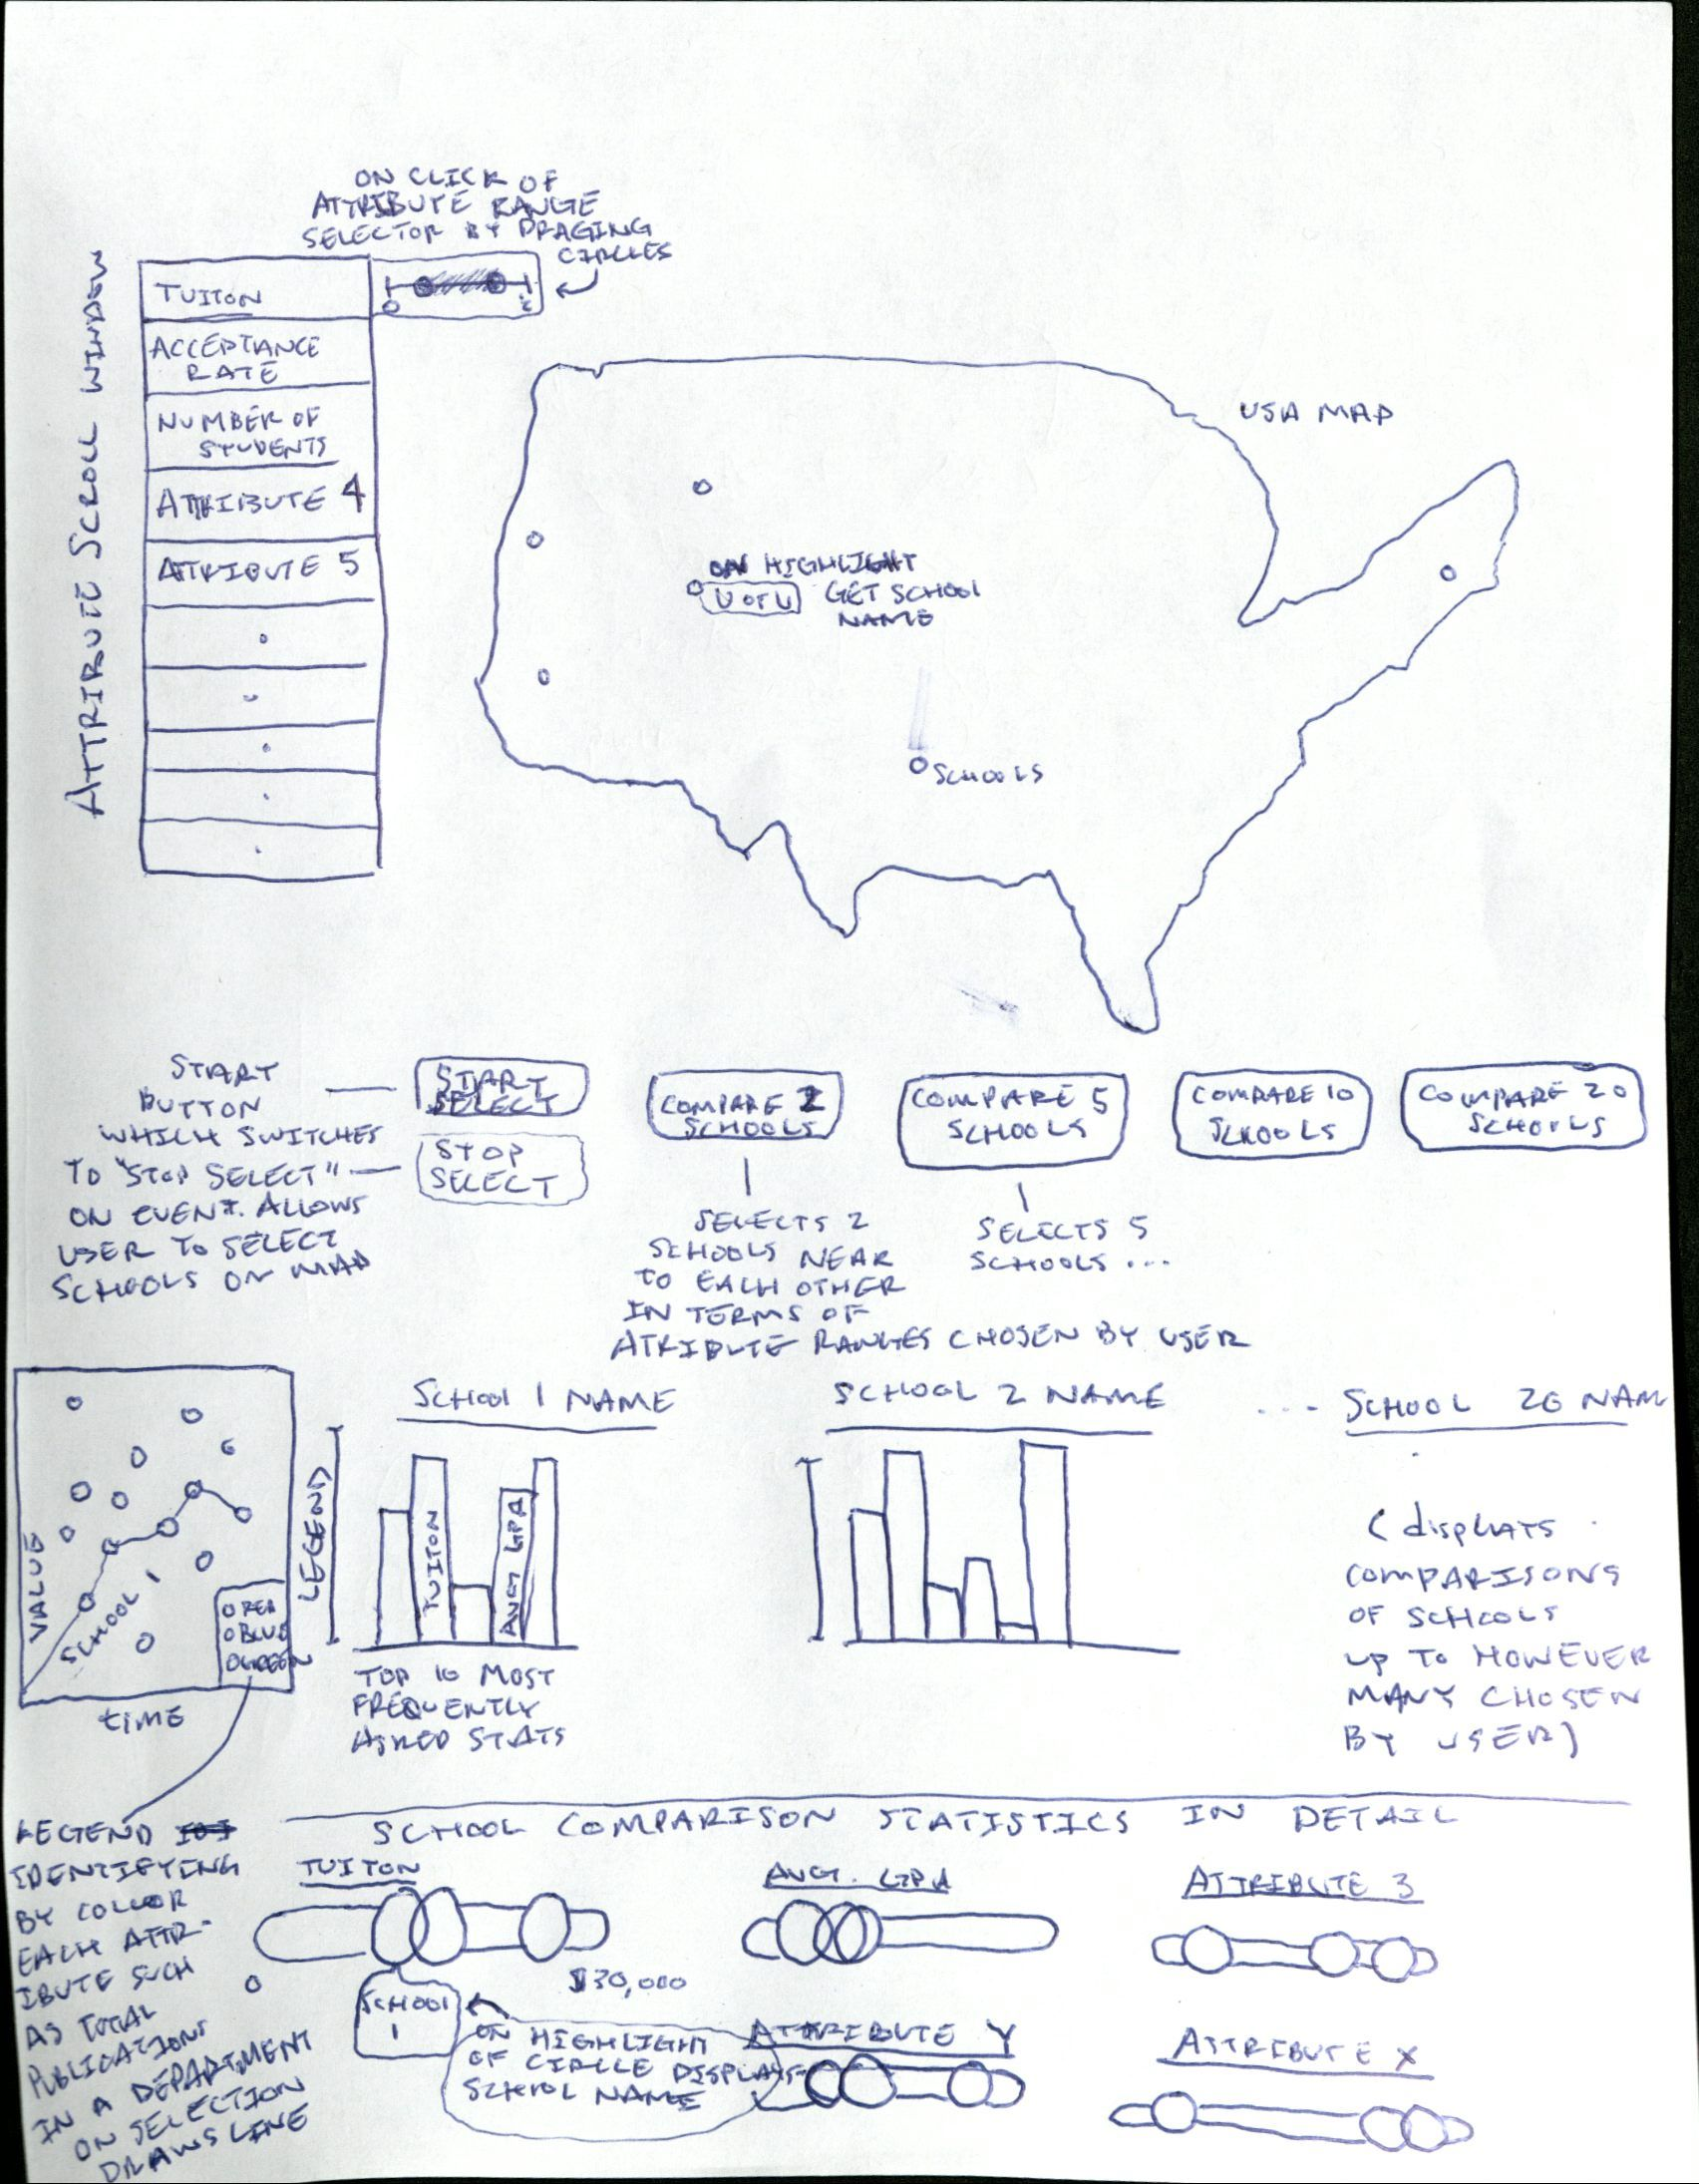
\includegraphics[width=.9\linewidth]{visualizationSketch.png}
}
\label{visualization sketch 1}
\end{figure}

\begin{figure}[H]
\centering{
\includegraphics[width=.9\linewidth]{barchart.png}
}
\label{visualization sketch 2}
\end{figure}

\begin{figure}[H]
\centering{
\includegraphics[width=.9\linewidth]{attributegauge.png}
}
\label{visualization sketch 3}
\end{figure}

\begin{figure}[H]
\centering{
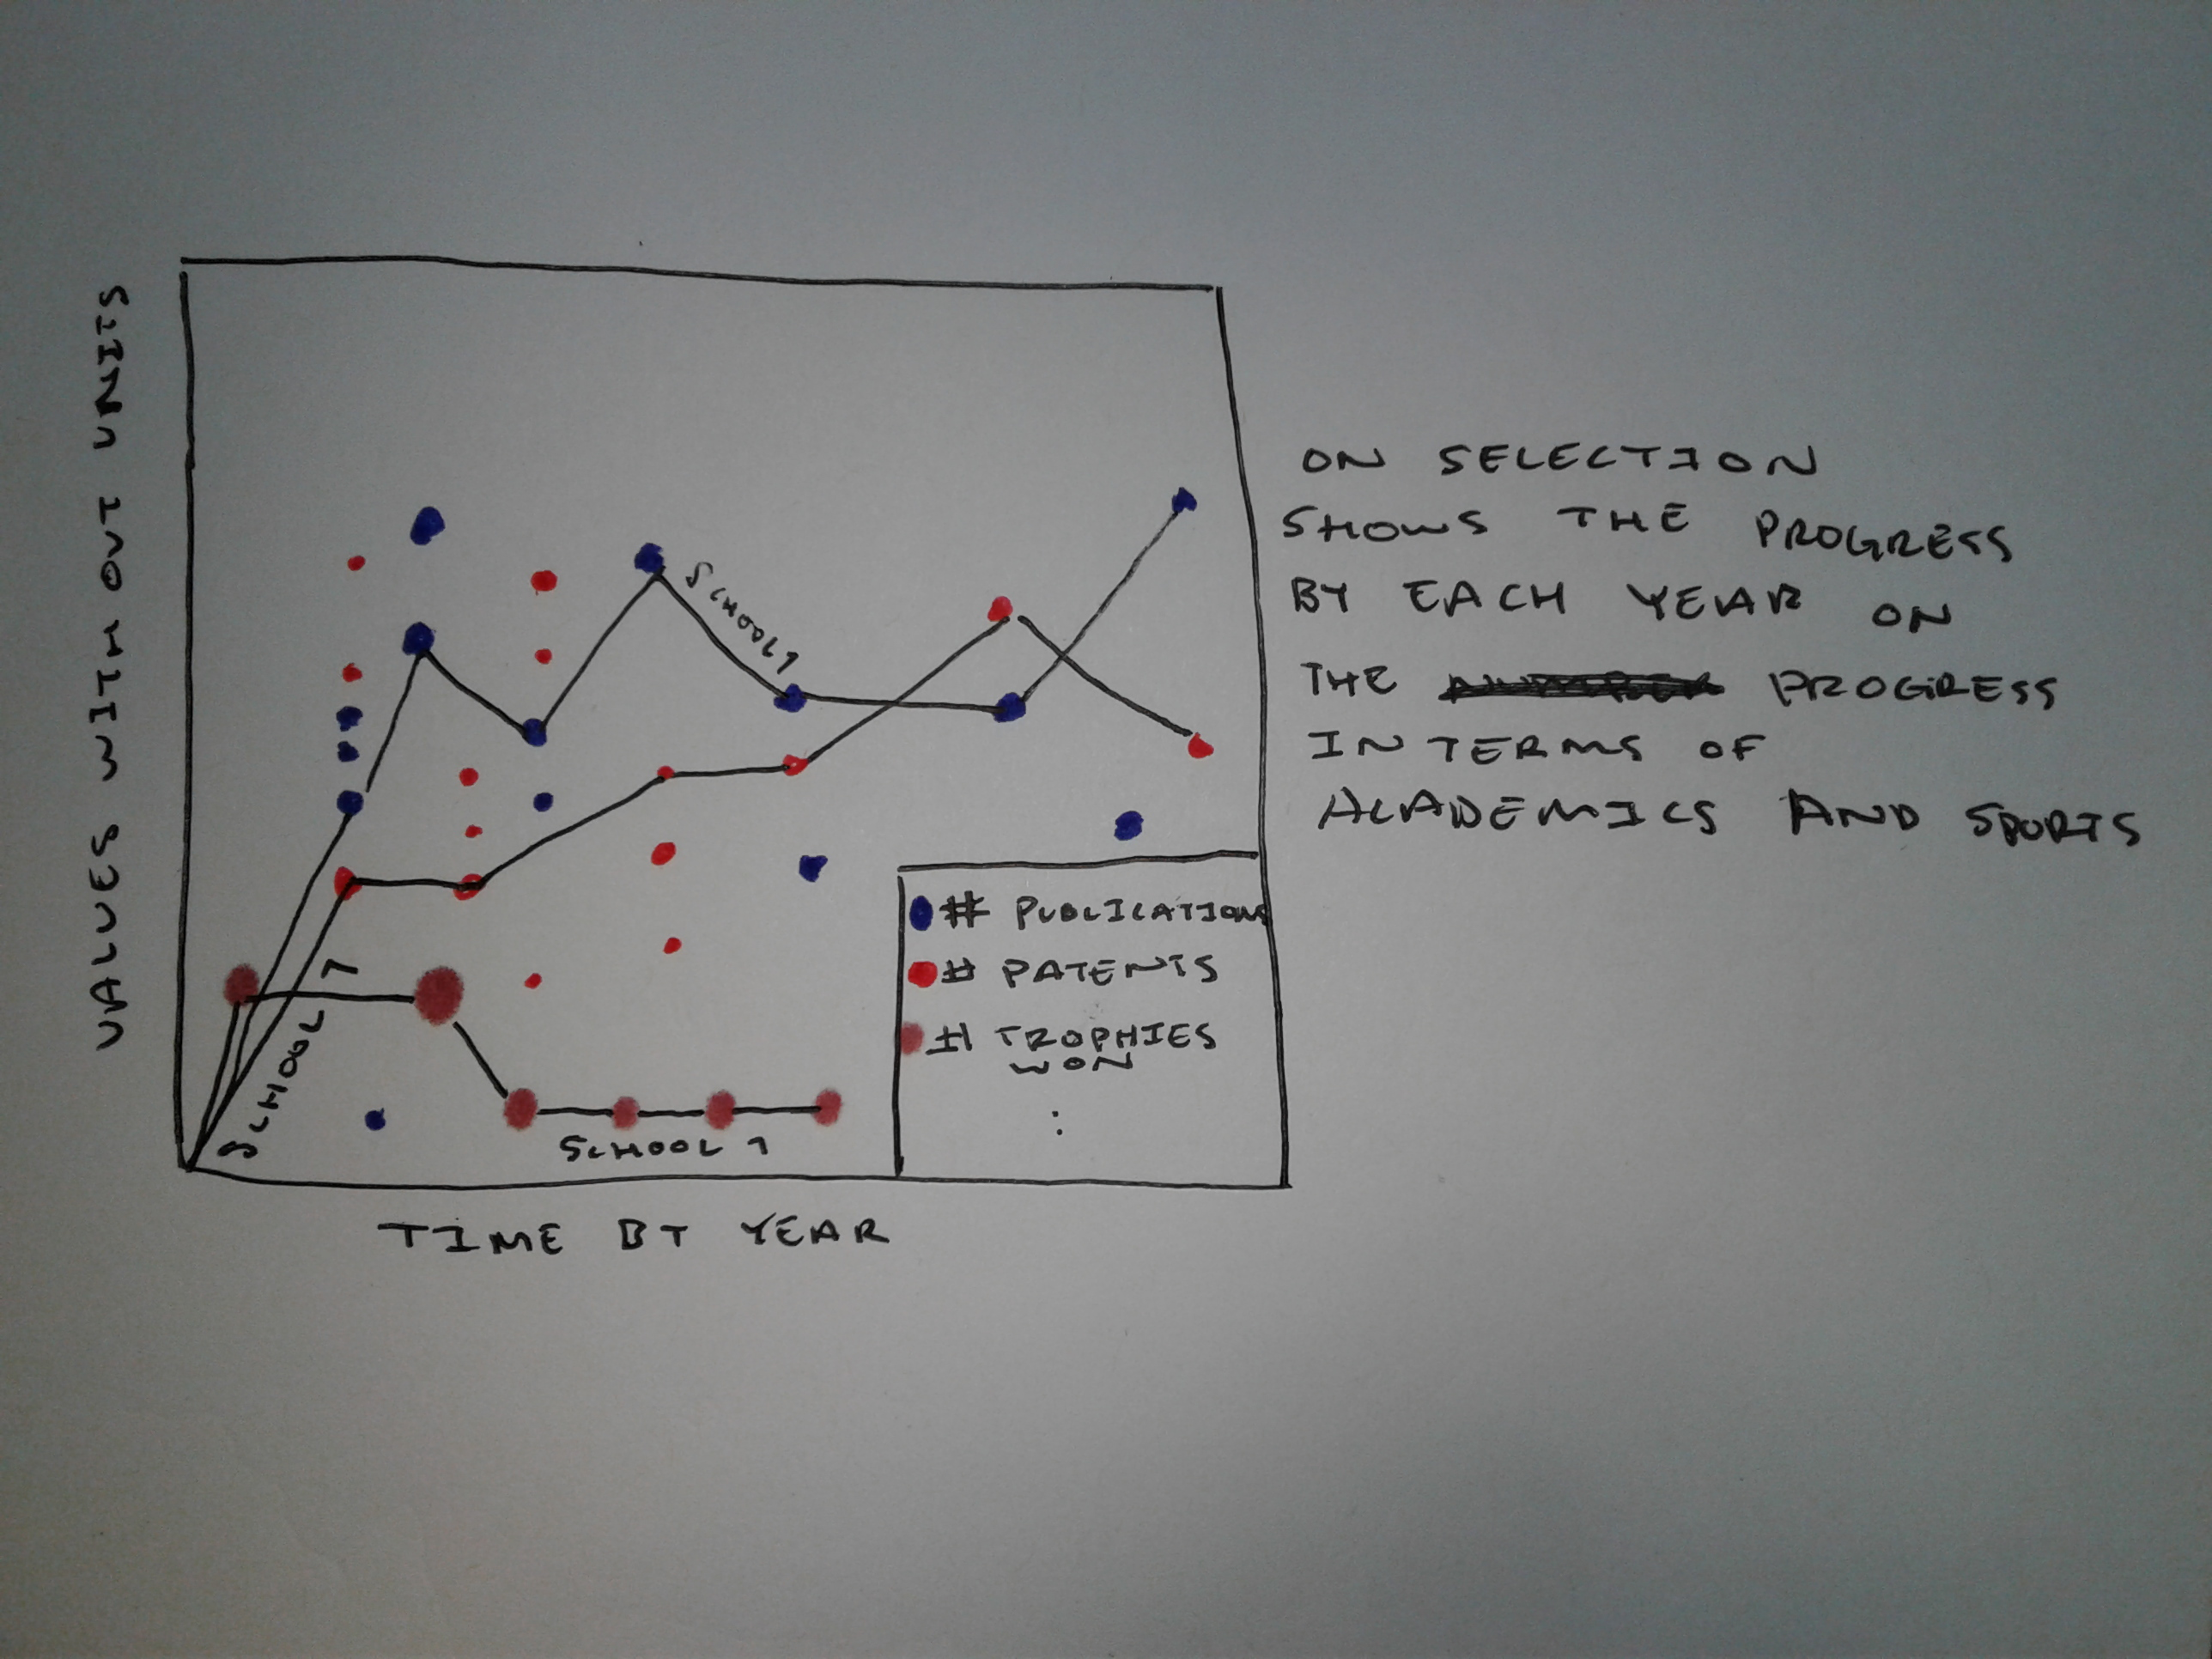
\includegraphics[width=.8\linewidth]{pointgraph.png}
}
\label{visualization sketch 4}
\end{figure}
  \subsection{Must-Have Features}\textbf{ List the features without which you would consider your project to be a failure.}
  Necessary visualizations and features include a map projection, hoverable and clickable points on the map for schools, legend with school statistics, click feature for each school statistic in the legend which opens a range selector in which one drags to points along a legend to represent what range to be considered, the option to select specific schools to compare, the option to compare a preset number of similar schools which fall into the user defined features of interest and their ranges, histograms for each selected school displaying it's specific attributes, a more detailed set of all features for each school consisting of oval bars representing an attribute's range and circles for the value of each selected school.

\subsection{Optional Features}\textbf{ List the features which you consider to be nice to have, but not critical.}
The feature which we feel nice to have would be to provide a visualization similar to GapMinder by Hans Rosling which was discussed in the class. Using this type of visualization we would be able to show the change in the school's performance over time.
The attributes we would consider are academic progress in terms of patents, publications, sports, endowment etc.

\vspace{5em}
\subsection{Project Schedule}{. Make sure that you plan your work so that you can avoid a big rush right before the final project deadline, and delegate different modules and responsibilities among your team members. Write this in terms of weekly deadlines.}
\begin{itemize}
\item Week 1 after proposal - Mine data from the sources
\item Week 2 - Map projections with Universities plotted
\item Week 3 -  Attribute selection Legend and selection comparison
\item Week 4 - Guage visualizations for selected universities
\item Week 5 - Work on GapMinder type visualization
\end{itemize}


\section{Peer Feedback}

\textbf{Feedback Group:}
\begin{itemize}
\item Shane Brown (u0852900)
\item Sigmund Chow (u0597938)
\item My Huynh (u0729654)
\end{itemize}

We found the feedback given very helpful and informative. Discussing our project illuminated aspects that were convoluted, allowing for new approaches to be either recommended by our reviewers or derived by us. Below are the suggestions or resolved confusions which we believe will provide for a more informative and intuitive visualization:
\begin{enumerate}
\item \textbf{Issue}:The bar charts for each school selected by the user add an extra component of confusion by grouping all top ten attributes for each school since attributes do not share the same units so height comparison is meaningless.
  
  \textbf{Solution}: We have decided to instead of creating a bar chart for each school we can better preserve the main goal of school comparison by making ten bar charts for each of the ``top ten first asked school attribute'' within which is a bar for each of the schools selected by the user. By doing so the user will be able to see how well any of the selected schools performs with respect to the other schools.
\item \textbf{Issue}: There is a level of redundancy by adding a ``Start'' and ``Stop'' button for when a user decides to select a school on the map.

  \textbf{Solution}: It was suggested instead the may select a school on the map which triggers the event of having that schools histogram as well as more detailed attributes to be displayed. After selecting a number of schools the comparisons between schools will all be displayed lower. The User can then remove a school by again selecting the school on the map or selecting a small ``x'' icon by the schools name lower down.

\item \textbf{Issue}: After explaining the attribute comparison in which a range, defined by the max and min value of the selected schools attributes, and each of the selected schools displayed within that range as a circle it was pointed out to us that as more schools are selected it will be difficult to maintain an understanding of how a school falls into a national perspective, i.e. if the range changes for the selected schools picking top 5 worst schools might look similar to the top 5 best schools.

  \textbf{Solution}: We can decided that not only would it be more informative but clearer to add to each attribute comparison in the ``detailed'' section two ranges: the first defined by the domain of the schools selected and the second defined by all schools. In this way as a user selects schools they will be able to see how a school from their selection performs with respect to the other selected schools as well as how the school compares nationally. To better illuminate this on the national scale we will also put a marker along the range indicating national average.
  
  

\end{enumerate}

\subsection{Other changes decided on}

We no longer will include the option to compare a preset number of schools. Our incentive for this is due to the ambiguity on which schools to select from the total range of each and between all attributes. We are also considering including a protip functionality on which where rather than only displaying the schools name when mousing over it's representative circle on the map it also displays in plain text the exact values of the top ten most asked questions about a school such as ranking, tuition, average acceptance rate, and so on. A sketch is given below on the direction we intend to take this project.

\begin{figure}[H]
\centering{
\includegraphics[width=.8\linewidth]{redesignedprojectvisualization.png}
}
\label{Redesigned Project Visualization}
\end{figure}


\section{Data Processing }

\section{Meetings With the TA}

\section{Obstacles, Improvements, Added Features, and Design Changes}

\subsection{Added Features}
While implementing our design we realized certain functionality was needed to make our visualization more dynamic and accessible. One such feature was the ability to deselect an attribute after having been selected by the brush selection. Originally a user was able to select multiple attributes in order to narrow down colleges of interest which fell into the value ranges desired. However if the user wished to no longer narrow the colleges displayed on the map for some attribute they would have to manually brush select the attributes entire range. Because of this we added the ability for the user to select again an attribute, after which that attributes range was rest to incorporate all values. 

\subsection{Design Changes}
While developing our visualization certain design changes were made to avoid a clutter as well as allow a more immediately understandable user interface. Specifically, our original design had intended to include all data from the data collected. Including all attributes however would not be practical due to the amount of attributes each college has. Instead we therefore sided with choosing key features applicants search when selecting schools. As a result of having less attributes we therefore no longer needed a scroll feature but instead could stack the attributes below the map and allow each attribute it's own brush selection bar to determine value range.

\section{To Do}
\begin{itemize}
\item Legend indicating school and attribute chosen.
\item Selected schools displayed in attribute range scale
\item Aesthetic touches
\item Comment Code
\item Zoom functionality to map with counties 
\end{itemize}


\end{document}
%%% Local Variables:
%%% mode: latex
%%% TeX-master: t
%%% End:

